\section{\iflanguage{english}{Methodology}{Herangehensweise}}
\label{sec:methodology}

in order to be able to understand the issue happening underneath the training procedure of neural networks we need to define our methodology to do so.

\subsection{Neural Network Architectures}

To evaluate the effects of different neural network designs on plasticity, three commonly used architectures are considered throughout this project: a Multi-Layer Perceptron (MLP), a Convolutional Neural Network (CNN), and a Vision Transformer (ViT). These architectures were selected because they represent three fundamentally different approaches to feature extraction and representation learning, allowing the investigation of whether plasticity-related phenomena are architecture-dependent.

\subsubsection{Multi-Layer Perceptron (MLP)}

The MLP consists of two fully connected hidden layers. Unless otherwise specified, each hidden layer contains 512 neurons. For the network width scaling experiment presented later in this report, the hidden layer width is varied to investigate the relationship between model capacity and plasticity. In these experiments, a base width of 16 neurons is multiplied by scaling factors of 1, 2, 4, 8, 12, and 16, resulting in progressively wider networks.

\subsubsection{Convolutional Neural Network (CNN)}

The CNN architecture consists of two convolutional layers followed by two fully connected layers. The first convolutional layer employs $5 \times 5$ kernels, while the second uses $3 \times 3$ kernels. Both convolutional layers contain 64 feature maps. The extracted features are then processed by two fully connected layers, each containing 256 hidden units before producing the final output.

\begin{figure}[htbp]
\centering
% Replace with reproduced Figure 1
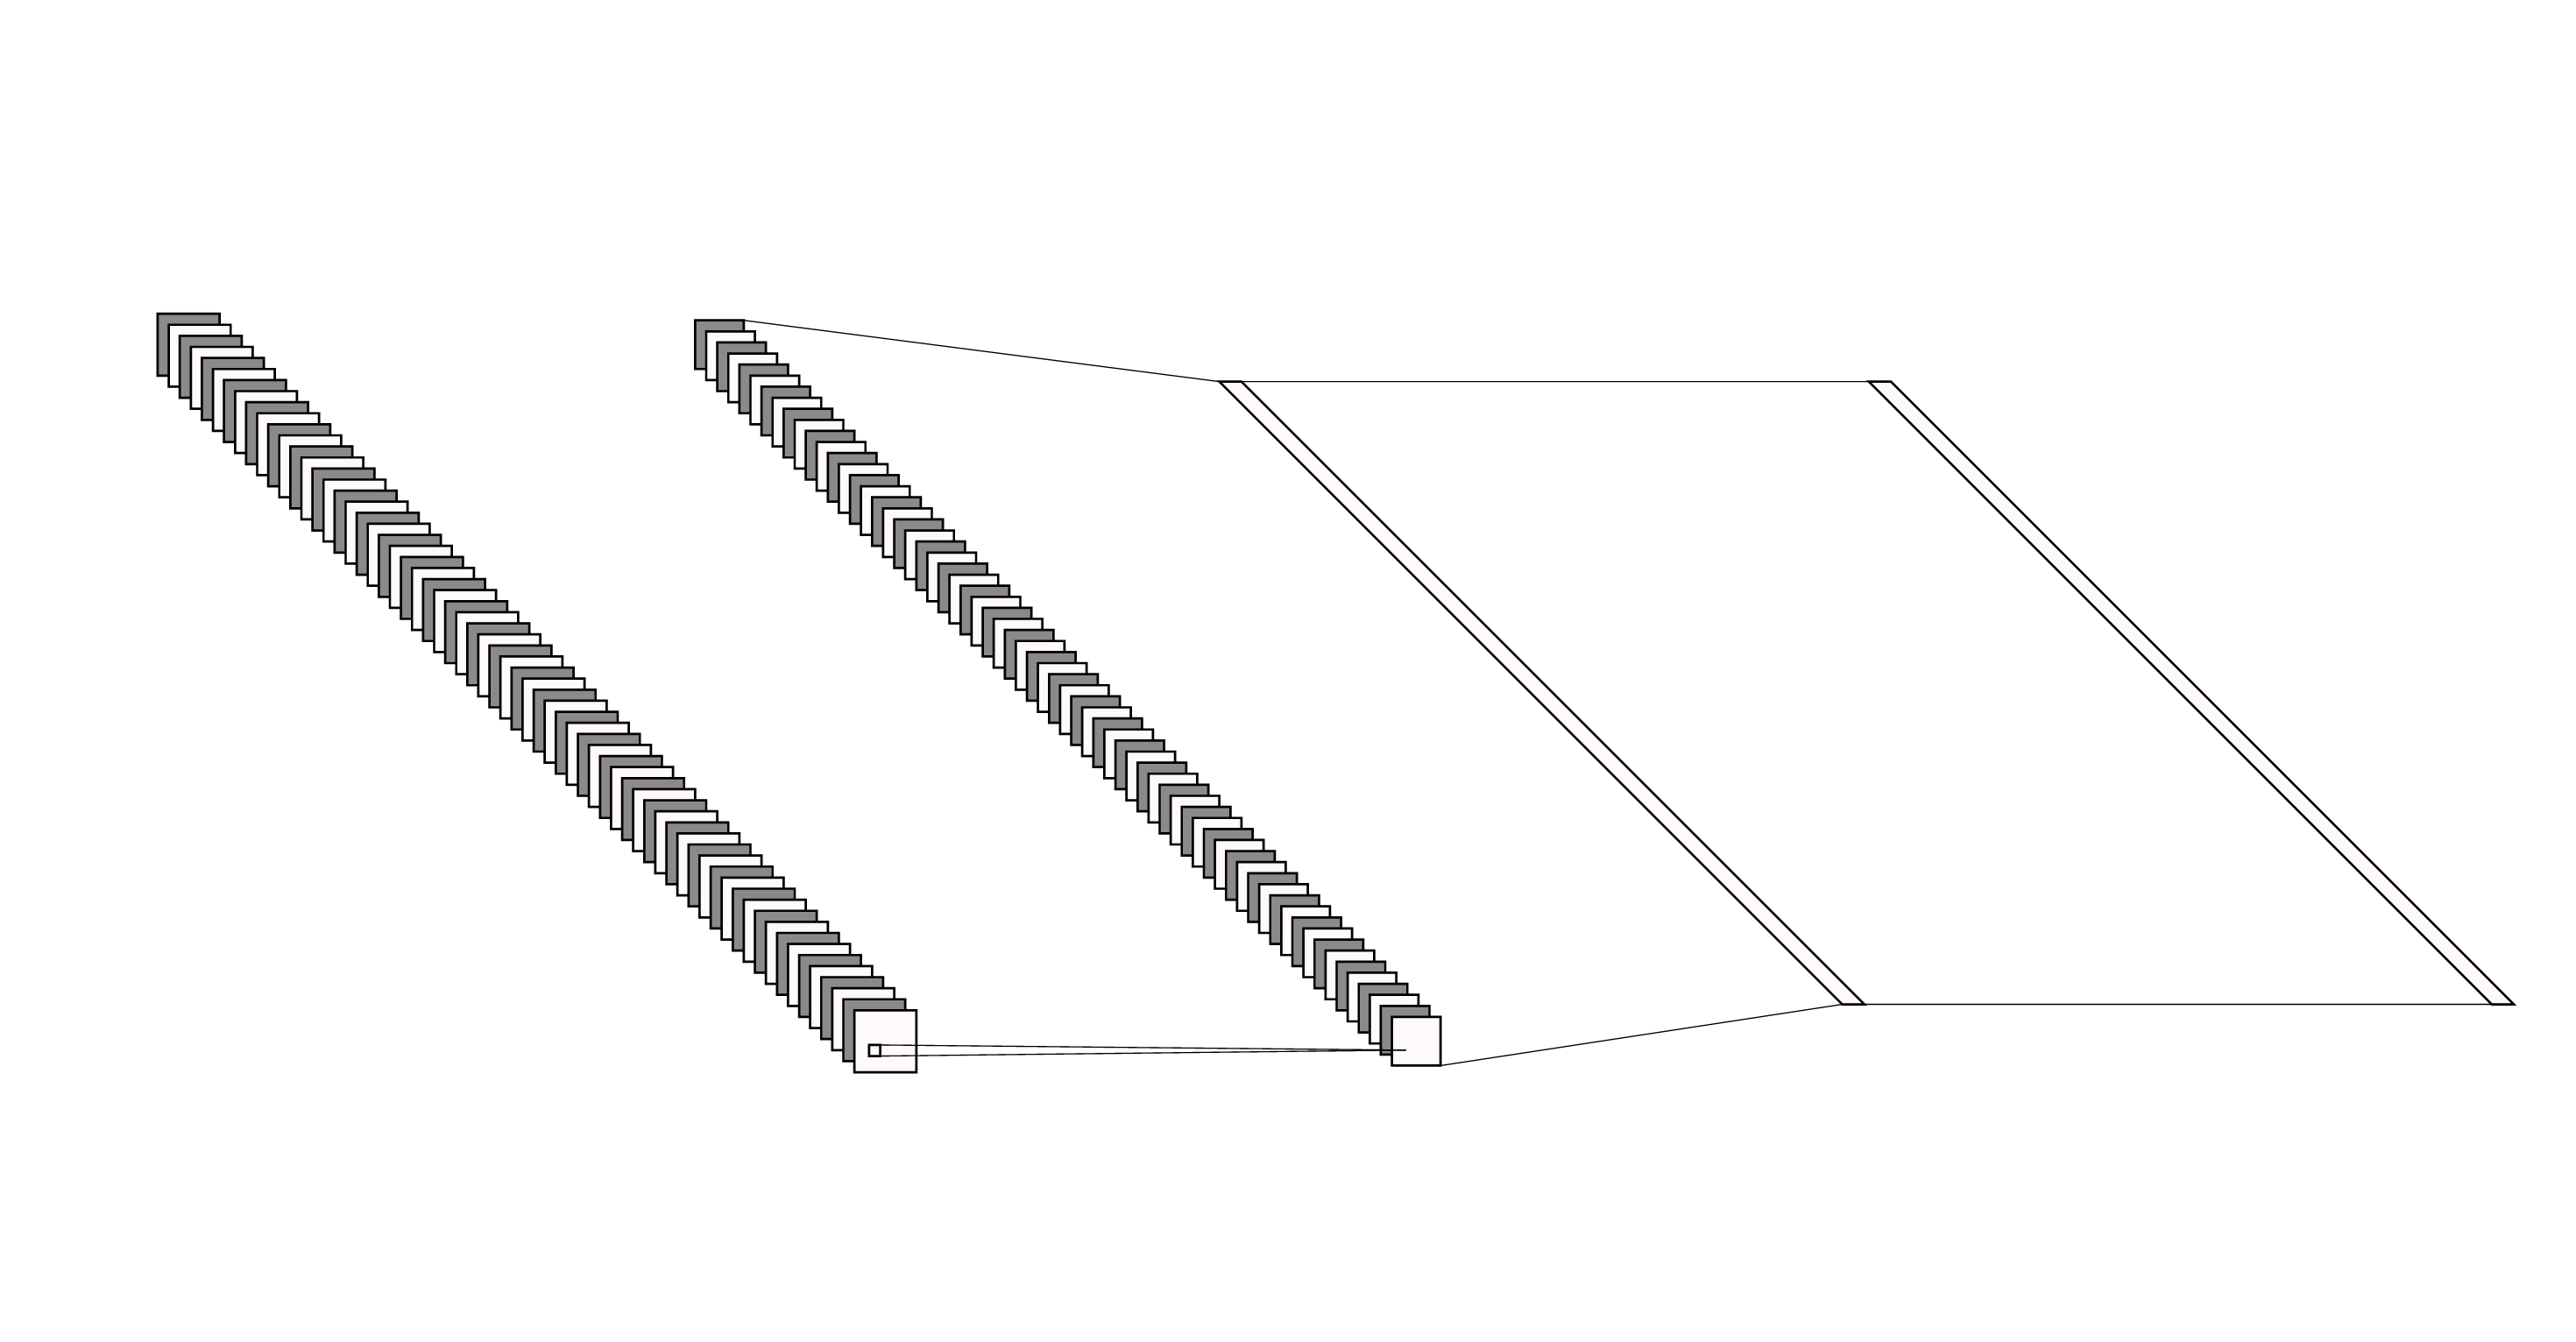
\includegraphics[width=0.9\textwidth]{assets/nn.png}
% \fbox{\rule{0pt}{2.6in}\rule{0.85\linewidth}{0pt}}
\caption{CNN on MNIST.}
\label{fig:cnn_mnist}
\end{figure}

% \subsubsection{Vision Transformer (ViT)}

% The Vision Transformer implementation follows the architecture proposed by \citet{dosovitskiy2020image}. Images are first divided into patches of size $3 \times 3$, which are embedded into a feature representation before being processed by a transformer encoder. The model uses an embedding dimension of 256, a feed-forward network dimension of 1024, a single transformer encoder block, and a dropout rate of 0.1. Unlike models initialized from pretrained weights, all parameters are trained from scratch during every experiment.

\begin{figure}[t]
    \centering
    %%%%%%%%%%%%%%%%%%%%%%%%%%%%%%%%%%%%%%%%%%%%%%%%%%%%%%%%%%%%%%%
    % Replace the following line with your architecture figure.
    %
    % Example:
    % \includegraphics[width=\textwidth]{figures/network_architectures.pdf}
    %
    \fbox{\rule{0pt}{6cm}\rule{0.95\textwidth}{0pt}}
    %%%%%%%%%%%%%%%%%%%%%%%%%%%%%%%%%%%%%%%%%%%%%%%%%%%%%%%%%%%%%%%
    \caption{Overview of the three neural network architectures used throughout this work: (a) Multi-Layer Perceptron (MLP), (b) Convolutional Neural Network (CNN), and (c) Vision Transformer (ViT). The figure illustrates the high-level structure of each architecture and highlights their different approaches to feature extraction and representation learning.}
    \label{fig:network_architectures}
\end{figure}

\subsection{Datasets}

We will be using the MNIST and CIFAR-10 datasets throughout the experiments. These datasets are among the most widely used benchmarks for image classification and provide two complementary levels of visual complexity. The MNIST dataset consists of 70,000 grayscale images of handwritten digits (60,000 training and 10,000 testing images), where each image has a resolution of 28 × 28 pixels and belongs to one of ten digit classes (0–9). Due to its simplicity, MNIST is commonly used for evaluating learning algorithms and analyzing optimization behaviour.

The CIFAR-10 dataset contains 60,000 colour images (50,000 training and 10,000 testing images), each with a resolution of 32 × 32 pixels and belonging to one of ten object categories, including airplanes, automobiles, birds, cats, deer, dogs, frogs, horses, ships, and trucks. Compared to MNIST, CIFAR-10 presents a substantially more challenging classification task because of its greater visual diversity, colour information, and more complex object features. Using both datasets enables the evaluation of neural network plasticity under learning tasks of varying complexity while maintaining a consistent ten-class classification setting.
\begin{table}[h]
\centering
\caption{Datasets used throughout the experiments.}
\label{tab:datasets}
\begin{tabular}{lcccc}
\toprule
Dataset & Image Size & Channels & Classes & Training / Test \\
\midrule
MNIST & $28 \times 28$ & 1 (Grayscale) & 10 & 60,000 / 10,000 \\
CIFAR-10 & $32 \times 32$ & 3 (RGB) & 10 & 50,000 / 10,000 \\
\bottomrule
\end{tabular}
\end{table}

\subsection{Measuring Plasticity}

The primary objective of this work is not to maximize reinforcement learning performance, but rather to understand and quantify the phenomenon of plasticity loss. Therefore, a precise operational definition of plasticity is required.

Following \citet{lyle2023understanding}, plasticity is defined as the ability of a neural network to update its predictions in response to new learning signals. More formally, consider an optimization algorithm:
\begin{equation}
\mathcal{O} : (\theta,\ell) \mapsto \theta^{*},
\end{equation}

which takes a parameter vector $\theta$ and a loss function $\ell$ and returns updated parameters $\theta^{*}$. The resulting parameters need not correspond to a global optimum; for example, $\mathcal{O}$ may simply perform a fixed number of gradient descent steps.

To measure the flexibility of a network, a distribution over learning objectives is considered. In particular, \citet{lyle2023plasticity} define a family of regression objectives

\begin{equation}
\ell_{f,X}(\theta)
=
\mathbb{E}_{x \sim X}
\left[
\left(
f(\theta,x)-g{\omega}(x)
\right)^2
\right],
\end{equation}

where $g_{\omega}$ defines a randomly generated target function.

To construct challenging prediction targets that require the network to modify its predictions in arbitrary directions, the target function is transformed according to

\begin{equation}
g(x)
=
a
+
\sin
\left(
10^{5}f(x;\omega_0)
\right),
\end{equation}

where $\omega_0$ is sampled from the same initialization distribution as the network parameters.

The offset parameter $a$ is chosen to match the mean prediction of the network. This prevents the probe task from favouring randomly initialized networks whose outputs tend to be centered around zero.

The resulting objective measures how easily a trained network can adapt its predictions to new targets. Networks capable of rapidly minimizing this objective are considered highly plastic, whereas networks that struggle to adapt are considered to have lost plasticity.

\subsection{Loss Landscape Analysis}

To better understand the optimization behaviour and plasticity of neural networks, this work analyzes the geometry of the loss landscape throughout training. In particular, two complementary quantities are investigated: the Hessian matrix of the loss function and the gradient covariance matrix. Together, these metrics provide insight into the curvature of the optimization landscape and the similarity of gradient directions across different training samples.

The Hessian matrix describes the second-order curvature of the loss function with respect to the network parameters. For a neural network with parameters $\theta$ and loss function $\ell(\theta)$, the Hessian is defined as

\begin{equation}
    H_{\ell}(\theta)=\nabla_{\theta}^{2}\ell(\theta)\in\mathbb{R}^{d\times d},
\end{equation}

where $d=|\theta|$ denotes the total number of trainable parameters. Since the Hessian is generally a very large matrix, its eigenspectrum is analyzed instead,

\begin{equation}
    \Lambda(H_{\ell}(\theta))
    =
    \left(
    \lambda_1,\lambda_2,\ldots,\lambda_d
    \right),
    \qquad
    \lambda_1\geq\lambda_2\geq\cdots\geq\lambda_d.
\end{equation}

The eigenvalues quantify the curvature of the loss landscape along different directions in parameter space, while the corresponding eigenvectors indicate these principal directions of curvature. The largest eigenvalue is commonly used as a measure of the sharpness of the loss landscape, whereas the ratio between the largest and smallest eigenvalues (the condition number) provides an indication of the numerical conditioning of the optimization problem. Poor conditioning generally results in slower convergence and more difficult optimization.

\begin{figure}[t]
    \centering
    %%%%%%%%%%%%%%%%%%%%%%%%%%%%%%%%%%%%%%%%%%%%%%%%%%%%%%%%%%%%%%%
    % Replace with Hessian illustration
    %
    % Example:
    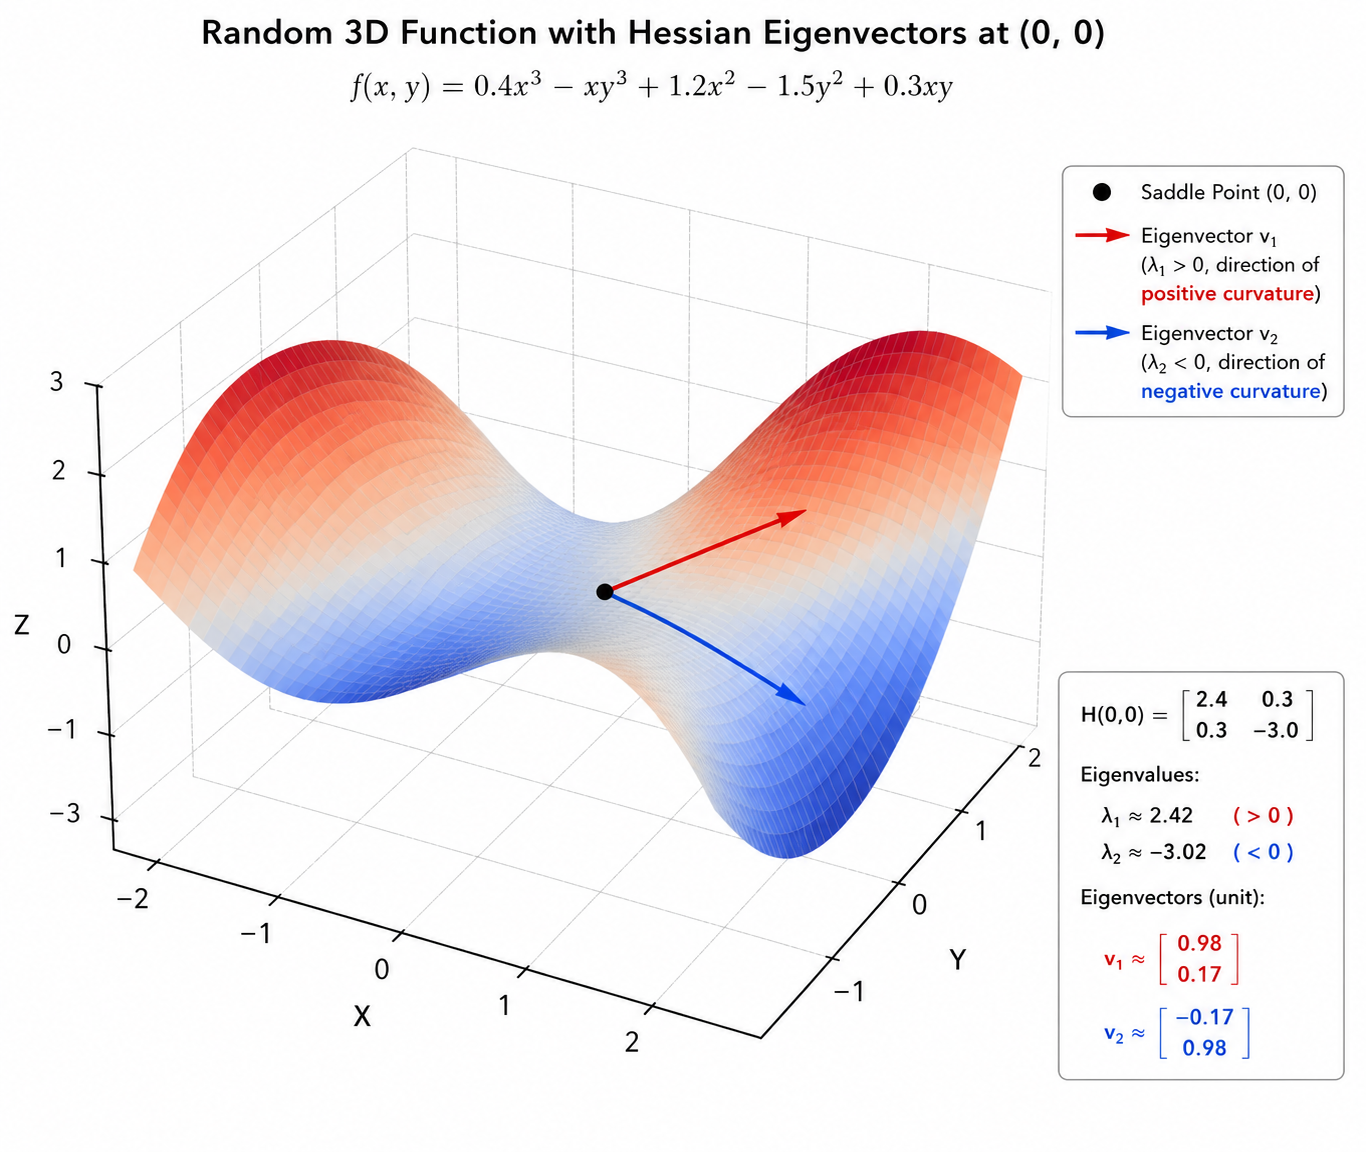
\includegraphics[width=0.75\textwidth]{assets/hessian_curvature.png}
    %
    % \fbox{\rule{0pt}{7cm}\rule{0.85\textwidth}{0pt}}
    %%%%%%%%%%%%%%%%%%%%%%%%%%%%%%%%%%%%%%%%%%%%%%%%%%%%%%%%%%%%%%%
    \caption{Illustration of a loss landscape together with the principal eigenvectors of the Hessian matrix. The eigenvectors indicate the directions of maximum and minimum curvature, while the corresponding eigenvalues quantify the curvature along those directions.}
    \label{fig:hessian_landscape}
\end{figure}

In addition to local curvature, this work also studies the similarity between gradients computed from different training samples. Let $x_1,\ldots,x_k$ denote a randomly sampled mini-batch of training examples. The gradient covariance matrix is computed as

\begin{equation}
C_k[i,j]
=
\frac{
\left\langle
\nabla_{\theta}\ell(\theta,x_i),
\nabla_{\theta}\ell(\theta,x_j)
\right\rangle
}{
\left\|
\nabla_{\theta}\ell(\theta,x_i)
\right\|
\left\|
\nabla_{\theta}\ell(\theta,x_j)
\right\|
},
\end{equation}

which corresponds to the cosine similarity between the gradients of every pair of training samples. Consequently, every entry of $C_k$ lies within the interval $[-1,1]$.

Positive values indicate that two samples produce similar parameter updates, suggesting cooperative learning and shared feature representations. Conversely, negative values imply that the corresponding gradients point in opposing directions, meaning that improving the performance on one sample may degrade the performance on the other. Such conflicting updates are commonly referred to as \emph{gradient interference} and have been identified as an important factor affecting plasticity and continual learning.

Finally, the rank and overall structure of the gradient covariance matrix are examined throughout training. A low-rank covariance matrix indicates that many gradients lie within a small subspace of the parameter space, revealing shared optimization directions across the dataset. Visualizing this matrix as a heatmap further exposes clusters of highly correlated or anti-correlated gradients, providing additional insight into how the network organizes its internal representations as learning progresses.

\subsection{Experimental Environments}

To carry out the experiments in this project, we do not use a large-scale reinforcement learning benchmark, but rather toy environments to create controlled datasets in which plasticity can be measured reliably.

To achieve this, the methodology proposed by \citet{lyle2023understanding} converts standard supervised learning datasets into Markov Decision Processes (MDPs). This design provides a controlled setting where the effects of plasticity loss can be isolated from other challenges commonly encountered in reinforcement learning.

The experiments use the MNIST and CIFAR-10 datasets and consider three environment variants.

\subsubsection{EasyMDP}

EasyMDP corresponds to the true-label setting.

Each image is associated with its original dataset label. The objective of the agent is therefore identical to standard classification. The environment serves as a baseline in which the network learns meaningful representations from naturally structured targets.

\subsubsection{HardMDP}

HardMDP corresponds to the random-label setting.

Before training begins, a random label is assigned independently to each image. Consequently, images belonging to the same class may receive entirely different labels.

For example, one image of the digit $7$ may be assigned label $5$, while another image of the $7$ may be assigned label $2$.

This environment removes the underlying structure of the dataset and forces the network to memorize arbitrary associations. The setting is intentionally difficult and is used to investigate how plasticity evolves under extreme memorization demands.

\subsubsection{Sparse-reward MDP}

Sparse-reward MDP corresponds to the reinforcement learning setting used in the original paper.

In this environment, the agent receives a reward only when it selects the correct action in a designated goal state. In the experiments, state $9$ is treated as the rewarding state.

The agent must therefore learn value estimates for all states and propagate reward information through the value function. Unlike EasyMDP and HardMDP, this environment introduces sparse rewards and temporal-difference learning, thereby capturing the essential characteristics of reinforcement learning.

% \subsection{Example Q-Value Representation}

% The following table illustrates the learned Q-value structure used in the environments. Numerical values are placeholders and should be replaced with the actual experimental results.

% \begin{table}[htbp]
% \centering
% \caption{Example Q-value table for EasyMDP.}
% \begin{tabular}{c|cccccccccc}
% & 0&1&2&3&4&5&6&7&8&9\
% \hline
% 0&0.1&0.2&0.3&0.4&0.5&0.6&0.7&0.8&0.9&1.0\
% 1&0.1&0.2&0.3&0.4&0.5&0.6&0.7&0.8&0.9&1.0\
% 2&0.1&0.2&0.3&0.4&0.5&0.6&0.7&0.8&0.9&1.0\
% 3&0.1&0.2&0.3&0.4&0.5&0.6&0.7&0.8&0.9&1.0\
% 4&0.1&0.2&0.3&0.4&0.5&0.6&0.7&0.8&0.9&1.0\
% 5&0.1&0.2&0.3&0.4&0.5&0.6&0.7&0.8&0.9&1.0\
% 6&0.1&0.2&0.3&0.4&0.5&0.6&0.7&0.8&0.9&1.0\
% 7&0.1&0.2&0.3&0.4&0.5&0.6&0.7&0.8&0.9&1.0\
% 8&0.1&0.2&0.3&0.4&0.5&0.6&0.7&0.8&0.9&1.0\
% 9&0.1&0.2&0.3&0.4&0.5&0.6&0.7&0.8&0.9&1.0\
% \end{tabular}
% \end{table}

\subsection{Deep Q-Network Learning}

A Deep Q-Network (DQN) \citep{mnih2015human} is used throughout the experiments.

Although exact dynamic programming methods could be applied to represent the Q-values directly, such approaches would not allow investigation of the internal dynamics of neural network learning. Since the objective of this project is to study plasticity loss within neural networks, a function approximator is required.

The DQN learns action values according to the Bellman equation

\begin{equation}
Q(s,a)
=
r
+
\gamma
\max_{a’}
Q(s’,a’).
\end{equation}

The network parameters are optimized using stochastic gradient descent on the temporal-difference loss

\begin{equation}
L(\theta)
=
\left(
y
-
Q(s,a; \theta)
\right)^2,
\end{equation}

where

\begin{equation}
y =
r
+
\gamma
\max_{a’}
Q(s’,a’;\theta^{-})
\end{equation}

and $\theta^{-}$ denotes the target network parameters.

Algorithm~\ref{alg:dqn} summarizes the DQN training procedure.

\begin{algorithm}[H]
\caption{Deep Q-Learning with Experience Replay}
\label{alg:dqn}
\begin{algorithmic}[1]

\State Initialize replay memory $\mathcal{D}$ with capacity $N$
\State Initialize action-value network $Q(s,a;\theta)$ with random parameters $\theta$
\State Initialize target network $\hat{Q}(s,a;\theta^-)$ with $\theta^- \leftarrow \theta$

\For{episode $=1,\dots,M$}

    \State Receive initial state $s_1$
    \State Preprocess state to obtain $\phi_1=\phi(s_1)$

    \For{$t=1,\dots,T$}

        \State With probability $\epsilon$, select a random action $a_t$
        \State Otherwise select
        \[
            a_t=\arg\max_a Q(\phi_t,a;\theta)
        \]

        \State Execute $a_t$, observe reward $r_t$ and next state $s_{t+1}$

        \State Preprocess next state:
        \[
            \phi_{t+1}=\phi(s_{t+1})
        \]
        \State Store transition
        \[
            (\phi_t,a_t,r_t,\phi_{t+1})
        \]
        in replay memory $\mathcal{D}$

        \State Sample a random minibatch of transitions from $\mathcal{D}$
        \[
            (\phi_j,a_j,r_j,\phi_{j+1})
        \]
        \ForAll{sampled transitions}
            \If{transition is terminal}
                \State
                \[
                y_j=r_j
                \]
            \Else
                \State
                \[
                y_j=r_j+\gamma
                \max_{a'}
                \hat{Q}(\phi_{j+1},a';\theta^-)
                \]
            \EndIf
        \EndFor
        \State Perform one gradient descent step on
        \[
            \left(y_j-Q(\phi_j,a_j;\theta)\right)^2
        \]
        with respect to $\theta$

        \If{$t \bmod C = 0$}
            \State Update target network:
            \[
            \theta^- \leftarrow \theta
            \]
        \EndIf
    \EndFor
\EndFor

\end{algorithmic}
\end{algorithm}